% Created 2017-03-23 Thu 10:09
\documentclass[10pt,t,a4paper]{beamer}
\usepackage[utf8]{inputenc}
\usepackage[T1]{fontenc}
\usepackage{fixltx2e}
\usepackage{graphicx}
\usepackage{longtable}
\usepackage{float}
\usepackage{wrapfig}
\usepackage{rotating}
\usepackage[normalem]{ulem}
\usepackage{amsmath}
\usepackage{textcomp}
\usepackage{marvosym}
\usepackage{wasysym}
\usepackage{amssymb}
\usepackage{hyperref}
\tolerance=1000
\usetheme{BTH_msv}
\author{Mikael Svahnberg\thanks{Mikael.Svahnberg@bth.se}}
\date{2016-03-09}
\title{Development Process}
\hypersetup{
  pdfkeywords={},
  pdfsubject={},
  pdfcreator={Emacs 25.1.1 (Org mode 8.2.10)}}
\begin{document}

\maketitle

\section{Classroom}
\label{sec-1}
\begin{frame}[label=sec-1-1]{Software Engineering}
\begin{itemize}
\item IEEE std 610.12:1990 ``IEEE Standard Glossary of Software Engineering Terminology'':
\end{itemize}

\begin{block}{Software Engineering}
The application of a systematic, disciplined, quantifiable approach to the development, operation, and maintenance of software; that is, the application of engineering to software.
\end{block}
\end{frame}

\begin{frame}[fragile,label=sec-1-2]{Software Engineering Process}
 \begin{itemize}
\item \alert{Systematic}
\begin{itemize}
\item Pre-planned, not ad-hoc
\item Thorough
\item Repeatable
\end{itemize}
\item \alert{Disciplined}
\begin{itemize}
\item Following the plan
\item Eyes on target
\end{itemize}
\item \alert{Quantifiable}
\begin{itemize}
\item Measurable
\end{itemize}
\end{itemize}


\begin{itemize}
\item \alert{Development}
\begin{itemize}
\item \texttt{*this}
\end{itemize}
\item \alert{Operation}
\begin{itemize}
\item Deployment is an important part of SE, and must be planned accordingly.
\end{itemize}
\item \alert{Maintenance}
\begin{itemize}
\item 80\% -- 90\% of a system's life span is spent in maintenance.
\end{itemize}
\end{itemize}
\end{frame}
\begin{frame}[label=sec-1-3]{Process vs Project vs Product}
T. Gorschek, A.M. Davis, \emph{Requirements Engineering; In Search of the Dependent Variables}, Information and Software Tecnology 50(2008):67--75.

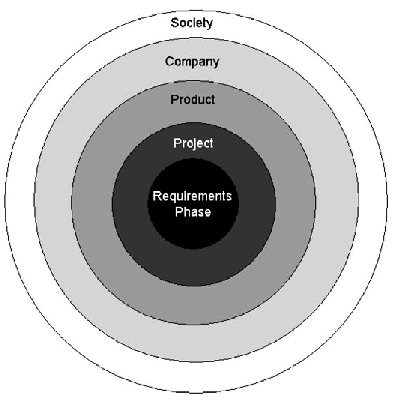
\includegraphics[height=5cm]{./IGorschek_Onion.pdf}

(+ Process, which is not visible in this figure but neatly bisects it.)
\end{frame}
\begin{frame}[shrink=15,label=sec-1-4]{Example of UML Process:}

\begin{block}{Dice Game Machine}
\begin{itemize}
\item On the Machine a player may login, logout or play the game.
\item When playing the game a player rolls two die. If the total number of points is greater than seven the player wins, otherwise the player loses.
\end{itemize}
\end{block}

\begin{block}{Construct}
\begin{itemize}
\item Use Case Diagrams
\item Use Cases
\item Conceptual Model
\item Class Diagram
\item Collaboration Diagram
\item Interaction Diagram
\item Flowcharts?
\item ?? What happened to testing ??
\end{itemize}
\end{block}
\end{frame}
\begin{frame}[label=sec-1-5]{Discussion}
\begin{itemize}
\item What is good with waterfall?
\item Where/How would you do design in Scrum?
\item Where would you do design in Kanban?
\item When should you use which process model?
\item What are their limitations?
\item Does it work to incrementally test a product like this?
\end{itemize}
\end{frame}



\begin{frame}[label=sec-1-6]{Project Planning}
\begin{itemize}
\item What do we need to know in order to plan something?
\item How do we put this together into a plan?
\end{itemize}
\end{frame}
\begin{frame}[label=sec-1-7]{Work Breakdown Structure}
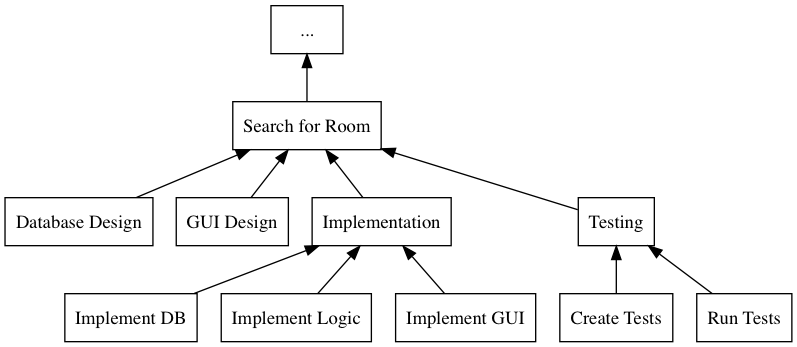
\includegraphics[width=.9\linewidth]{FWBSExample.png}
\end{frame}

\begin{frame}[fragile,shrink=60,label=sec-1-8]{GANTT}

 \begin{center}
\begin{tabular}{lllllllllll}
Feature & Tasks & Sub-Tasks & Effort & Start Date & End Date & Responsible & Spent Time & Progress & Projected Effort & Over/Undertime\\
\hline
Search for Room & Database Design &  &  &  &  &  &  &  & \verb~spent/progress~ & \verb~(est eff.) - (proj. eff)~\\
 & GUI Design &  &  &  &  &  &  &  &  & \\
 & Implementation & Implement DB &  &  &  &  &  &  &  & \\
 &  & Implement Logic &  &  &  &  &  &  &  & \\
 &  & Implement GUI &  &  &  &  &  &  &  & \\
 & Testing & Create Tests &  &  &  &  &  &  &  & \\
 &  & Run Tests &  &  &  &  &  &  &  & \\
\end{tabular}
\end{center}


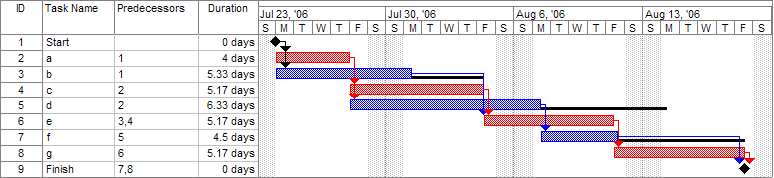
\includegraphics[width=.9\linewidth]{./IGANTT.png}
\end{frame}

\begin{frame}[label=sec-1-9]{Tracking Progress}
\begin{itemize}
\item Reporting \emph{Time} or reporting \emph{Progress}
\begin{itemize}
\item Amount of time/money spent
\item Delivered LOC?
\item Completed Tasks?
\end{itemize}
\item Earned Value Charts
\begin{itemize}
\item Planned cost (value)
\item Actual cost
\item Earned Value
\end{itemize}
\end{itemize}
\end{frame}
\begin{frame}[fragile,label=sec-1-10]{Story Points}
 \begin{itemize}
\item An arbitrary measure of the size of a task
\item Typically uses a modification of a fibonacci sequence:
\begin{itemize}
\item \verb~1,2,3,5,13,40,100~
\end{itemize}
\item Use them to
\begin{itemize}
\item measure \emph{velocity} of your development team.
\item plan sprints accordingly
\end{itemize}
\end{itemize}
\end{frame}
\begin{frame}[label=sec-1-11]{Earned Value Charts: Planned}
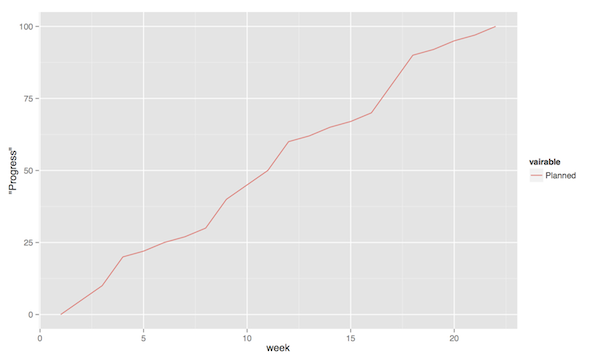
\includegraphics[width=.9\linewidth]{../Site/images/IEV_Planned.png}
\end{frame}

\begin{frame}[label=sec-1-12]{Earned Value Chart: Adding Actual Cost}
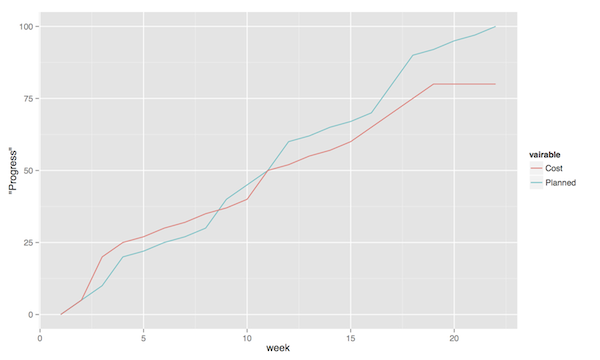
\includegraphics[width=.9\linewidth]{../Site/images/IEV_Cost.png}
\end{frame}

\begin{frame}[label=sec-1-13]{Earned Value Chart}
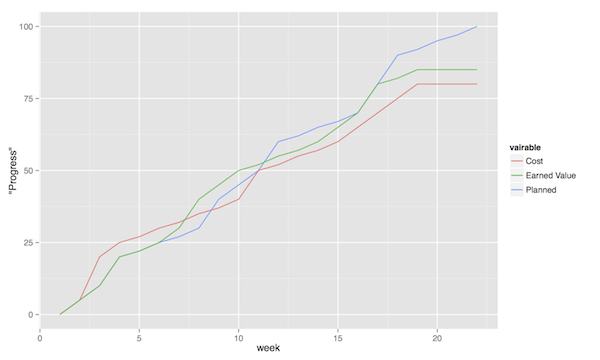
\includegraphics[width=.9\linewidth]{../Site/images/IEV_Earned.png}
\end{frame}

\begin{frame}[label=sec-1-14]{Burndown chart}
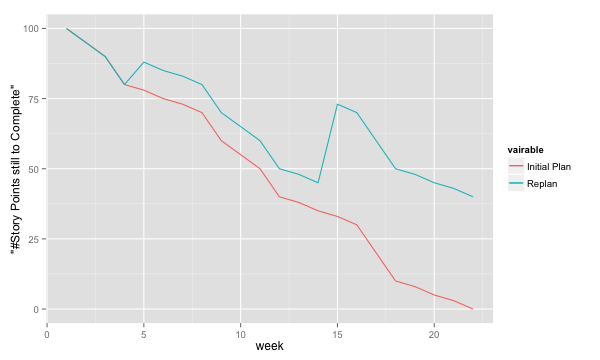
\includegraphics[width=.9\linewidth]{../Site/images/FBurndown_Replan.png}
\end{frame}

\begin{frame}[label=sec-1-15]{Risk Management}
\begin{itemize}
\item Identify risks
\item Develop plans to minimise their effect on a project
\item A risk is a probability that some adverse circumstance will occur
\begin{itemize}
\item Project risks affect schedule or resources
\item Product risks affect the quality or performance of the software being developed
\item Business risks affect the organisation developing or procuring the software
\end{itemize}
\item Monitor and mitigate risks
\end{itemize}
\end{frame}
% Emacs 25.1.1 (Org mode 8.2.10)
\end{document}